\documentclass[notes,serif]{beamer}
\usepackage{graphicx}
\usepackage{url}
\usepackage{clrscode}
\usepackage{amssymb,amsmath}

% You should run 'pdflatex' TWICE, because of TOC issues.

\mode<presentation>
{
  % A tip: pick a theme you like first, and THEN modify the color theme, and then add math content.
  % Warsaw is the theme selected by default in Beamer's installation sample files.

  %%%%%%%%%%%%%%%%%%%%%%%%%%%% THEME
  %\usetheme{AnnArbor}
  %\usetheme{Antibes}
  %\usetheme{Bergen}
  %\usetheme{Berkeley}
  %\usetheme{Berlin}
  %\usetheme{Boadilla}
  %\usetheme{boxes}
  %\usetheme{CambridgeUS}
  %\usetheme{Copenhagen}
  %\usetheme{Darmstadt}
  %\usetheme{default}
  %\usetheme{Dresden}
  %\usetheme{Frankfurt}
  %\usetheme{Goettingen}
  %\usetheme{Hannover}
  %\usetheme{Ilmenau}
  %\usetheme{JuanLesPins}
  %\usetheme{Luebeck}
  %\usetheme{Madrid}
  %\usetheme{Malmoe}
  %\usetheme{Marburg}
  %\usetheme{Montpellier}
  %\usetheme{PaloAlto}
  %\usetheme{Pittsburgh}
  %\usetheme{Rochester}
  %\usetheme{Singapore}
  %\usetheme{Szeged}
  \usetheme{Warsaw}

  %%%%%%%%%%%%%%%%%%%%%%%%%%%% COLOR THEME
  %\usecolortheme{albatross}
  %\usecolortheme{beetle}
  %\usecolortheme{crane}
  \usecolortheme{default}
  %\usecolortheme{dolphin}
  %\usecolortheme{dove}
  %\usecolortheme{fly}
  %\usecolortheme{lily}
  %\usecolortheme{orchid}
  %\usecolortheme{rose}
  %\usecolortheme{seagull}
  %\usecolortheme{seahorse}
  %\usecolortheme{sidebartab}
  %\usecolortheme{structure}
  %\usecolortheme{whale}

  %%%%%%%%%%%%%%%%%%%%%%%%%%%% OUTER THEME
  %\useoutertheme{default}
  %\useoutertheme{infolines}
  %\useoutertheme{miniframes}
  %\useoutertheme{shadow}
  %\useoutertheme{sidebar}
  %\useoutertheme{smoothbars}
  %\useoutertheme{smoothtree}
  %\useoutertheme{split}
  %\useoutertheme{tree}

  %%%%%%%%%%%%%%%%%%%%%%%%%%%% INNER THEME
  %\useinnertheme{circles}
  %\useinnertheme{default}
  %\useinnertheme{inmargin}
  %\useinnertheme{rectangles}
  %\useinnertheme{rounded}

  %%%%%%%%%%%%%%%%%%%%%%%%%%%%%%%%%%%

%  \setbeamercovered{transparent} % or whatever (possibly just delete it)
  \setbeamercovered{invisible} % or whatever (possibly just delete it)
  % To change behavior of \uncover from graying out to totally invisible, can change \setbeamercovered to invisible instead of transparent. apparently there are also 'dynamic' modes that make the amount of graying depend on how long it'll take until the thing is uncovered.

}


% Get rid of nav bar
\beamertemplatenavigationsymbolsempty

% Use short top
%\usepackage[headheight=12pt,footheight=12pt]{beamerthemeboxes}
%\addheadboxtemplate{\color{black}}{
%\hskip0.3cm
%\color{white}
%\insertshortauthor \ \ \ \
%\insertframenumber \ \ \ \ \ \ \
%\insertsection \ \ \ \ \ \ \ \ \ \ \ \ \ \ \ \ \  \insertsubsection
%\hskip0.3cm}
%\addheadboxtemplate{\color{black}}{
%\color{white}
%\ \ \ \
%\insertsection
%}
%\addheadboxtemplate{\color{black}}{
%\color{white}
%\ \ \ \
%\insertsubsection
%}

% Insert frame number at bottom of the page.
\usefoottemplate{\hfil\tiny{\color{black!90}\insertframenumber}}

\usepackage[english]{babel}
\usepackage[latin1]{inputenc}

\usepackage{times}
\usepackage[T1]{fontenc}

\title{Network Programming}
\subtitle{Lecture 5---Advanced Sockets I: \\ Raw Sockets and Datalink Access}

\author{Lei Wang\\ lei.wang@dlut.edu.cn}

\institute{Dalian University of Technology}

%\date{Date}
\date{Dec 15, 2008}

\subject{Talks}

\def\defn#1{{\color{red} #1}}

\begin{document}

\begin{frame}
  \titlepage
\end{frame}

\begin{frame}
  \frametitle{Part 3. Advanced Sockets I: \\ Raw Sockets and Datalink Access}
  \tableofcontents
\end{frame}

\section{Raw Socket}
\subsection{Introduction}
\begin{frame}
\frametitle{Introduction}

Raw sockets provide three features not provided by normal TCP and UDP sockets:
\begin{itemize}
  \item Raw sockets let us read and write ICMPv4, IGMPv4, and ICMPv6 packets. (\texttt{ping}, \texttt{mrouted})
  \item With a raw socket, a process can read and write IPv4 datagrams with an IPV4 protocol field that is not processed by the kernel.
  \item With a raw socket, a process can build its own IPv4 header using the \texttt{IP\_HDRINCL} socket option.
\end{itemize}
\end{frame}

\subsection{Raw Socket Creation, Output and Input}

\begin{frame}[containsverbatim]
\frametitle{Raw Socket Creation}
\begin{itemize}
  \item \texttt{SOCKET\_RAW}
{\scriptsize
  \begin{verbatim}
int     sockfd;

sockfd = socket(AF_INET, SOCK_RAW, protocol);
  \end{verbatim}
  \begin{flushleft}
  where protocol is one of the constants, \texttt{IPPROTO\_xxx}, such as \texttt{IPPROTO\_ICMP}.
  \end{flushleft}
}
  \item \texttt{IP\_HDRINCL} socket option
  \item \texttt{bind} can be called on the raw socket, but this is rare.
  \item \texttt{connect} can be called on the raw socket, but this is rare.
\end{itemize}
\end{frame}

\begin{frame}
\frametitle{Raw Socket Output}
\begin{itemize}
  \item Normal output is performed by calling \texttt{sendto} or \texttt{sendmsg} and specifying the destination IP address.
  \item If the \texttt{IP\_HDRINCL} option is \textbf{\emph{not}} set, the starting address of the data for the kernel to send specifies the first byte following the IP header because the kernel will build the IP header and prepend it to the data from the process.
  \item If the \texttt{IP\_HDRINCL} option is set, the starting address of the data for the kernel to send specifies the first byte of the IP header.
  \item The kernel fragments raw packets that exceed the outgoing interface MTU.
\end{itemize}
\end{frame}

\begin{frame}
\frametitle{Raw Socket Input}
Which received IP datagrams does the kernel pass to raw sockets? The following rules apply:
\begin{itemize}
  \item Received UDP packets and received TCP packets are never passed to a raw socket. (must be read at the datalink layer)
  \item Most ICMP packets are passed to a raw socket after the kernel has finished processing the ICMP message.
  \item All IGMP packets are passed to a raw socket after the kernel has finished processing the IGMP message.
  \item All IP datagrams with a protocol field that the kernel does not understand are passed to a raw socket.
  \item If the datagram arrives in fragments, nothing is passed to a raw socket until all fragments have arrived and have been reassembled.
\end{itemize}
\end{frame}

\begin{frame}
\frametitle{Raw Socket Input Contd.}
{\scriptsize
When the kernel has an IP datagram to pass to the raw sockets, all raw sockets for all processes are examined, looking for all matching sockets. A copy of the IP datagram is delivered to each matching socket. The following tests are performed for each raw socket and only if all three tests are true is the datagram delivered to the socket:

\begin{itemize}
  \item If a nonzero protocol is specified when the raw socket is created (the third argument to \texttt{socket}), then the received datagram's protocol field must match this value or the datagram is not delivered to this socket.
  \item If a local IP address is bound to the raw socket by \texttt{bind}, then the destination IP address of the received datagram must match this bound address or the datagram is not delivered to this socket.
  \item If a foreign IP address was specified for the raw socket by \texttt{connect}, then the source IP address of the received datagram must match this connected address or the datagram is not delivered to this socket.
\end{itemize}

Notice that if a raw socket is created with a protocol of 0, and neither \texttt{bind} nor \texttt{connect} is called, then that socket receives a copy of every raw datagram the kernel passes to raw sockets.
}
\end{frame}

\subsection{\texttt{ping} and \texttt{traceroute} Program}
\begin{frame}
\frametitle{\texttt{ping} Program}
\begin{itemize}
\item A \texttt{ping} program without suffering \textit{creeping featurism}.
\item Overview of the functions in the \texttt{ping} program.
\vskip 2em
 \begin{center}
  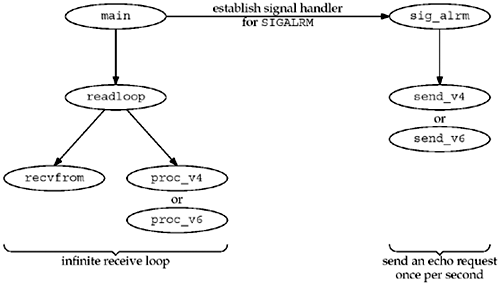
\includegraphics[width=.7\textwidth]{figs/28fig03.png}
  \end{center}
\end{itemize}
\end{frame}

\begin{frame}
\frametitle{\texttt{traceroute} Program}
\begin{itemize}
  \item \texttt{traceroute} lets us determine the path that IP datagrams follow from our host to other destination.
  \item Exploit the IPv4 TTL field, ICMP ``time exceeded in transit'' and ICMP ``port unreachable'' error.
  \item \texttt{IP\_HDRINCL} and \texttt{IP\_TTL}
\end{itemize}
\end{frame}

\section{Datalink Access}
\subsection{Introduction}
\begin{frame}
\frametitle{Datalink Access}
Providing access to the datalink layer for an application, with the following capabilities:
\begin{itemize}
  \item The ability to watch the packets received by the datalink layer, allowing programs such as \texttt{tcpdump} to be run on normal computer systems (as opposed to dedicated hardware devices to watch packets). (\textbf{\textit{promiscuous mode}})
  \item The ability to run certain programs as normal applications instead of as part of the kernel. For example, most Unix versions of an RARP server are normal applications that read RARP requests from the datalink (RARP requests are not IP datagrams) and then write the reply back to the datalink.
  \item Three common methods under Unix are: the BSD Packet Filter (BPF), the SVR4 Datalink Provider Interface (DLPI), and the Linux \texttt{SOCK\_PACKET} interface.
\end{itemize}
\end{frame}

\subsection{BPF, DLPI and Linux: \texttt{SOCK\_PACKET} and \texttt{PF\_PACKET}}
\begin{frame}
\frametitle{BSD Packet Filter (BPF)}
4.4BSD and many other Berkeley-derived implementations support BPF.
  \begin{center}
  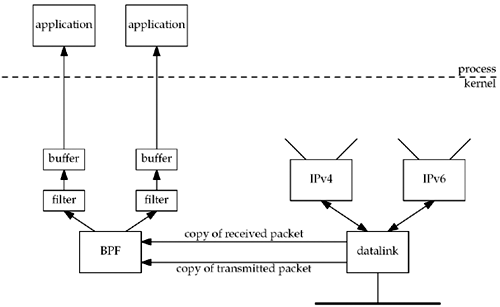
\includegraphics[width=.65\textwidth]{figs/29fig01.png}
  \end{center}
\end{frame}

\begin{frame}
\frametitle{Datalink Provide Interface (DLPI)}
SVR4 provides datalink access through DLPI.
  \begin{center}
  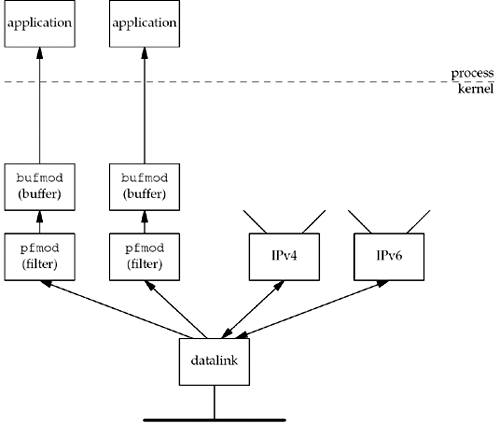
\includegraphics[width=.6\textwidth]{figs/29fig02.png}
  \end{center}
\end{frame}

\begin{frame}[containsverbatim]
\frametitle{Linux: \texttt{SOCK\_PACKET} and \texttt{PF\_PACKET}}
Two methods under Linux: 
\begin{itemize}
  \item \texttt{SOCK\_PACKET}: original, widely available but less flexible
  \item \texttt{PF\_PACKET}: newer method
\end{itemize}
{\scriptsize
\begin{verbatim}
/* newer systems*/
fd = socket(PF_PACKET, SOCK_RAW, htons(ETH_P_ALL));
      
/* older systems*/
fd = socket(AF_INET, SOCK_PACKET, htons(ETH_P_ALL));     
\end{verbatim}
}
\end{frame}

\subsection{\texttt{libpcap}: Packet Capture Library}
\begin{frame}
\frametitle{\texttt{libpcap}: Packet Capture Library}
\begin{itemize}
  \item \texttt{libpcap} provides implementation-independent access to the underlying packet capture facility provided by the OS.
  \item Currently, it supports only the reading of packets (although adding a few lines of code to the library lets one write datalink packets too on some systems).
  \item The library is available from \texttt{http://www.tcpdump.org/}.
\end{itemize}
\end{frame}

\subsection{\texttt{libnet}: Packet Creation and Injection Library}
\begin{frame}
\frametitle{\texttt{libnet}: Packet Creation and Injection Library}
\begin{itemize}
  \item \texttt{libnet} provides an interface to craft and inject arbitrary packets into the network.
  \item It provides both raw socket and datalink access modes in an implementation-independent manner.
  \item \href{http://www.packetfactory.net/libnet/}{\tt http://www.packetfactory.net/libnet/}
\end{itemize}
\end{frame}

\subsection{Example: Examining the UPD Checksum Field}
\begin{frame}
\frametitle{Example: Examining the UPD Checksum Field}
  \begin{center}
  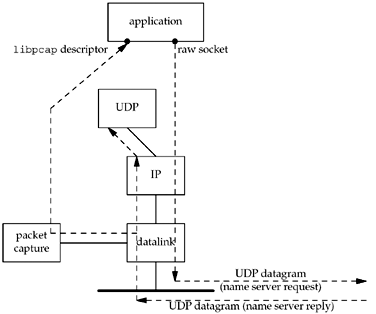
\includegraphics[width=.6\textwidth]{figs/29fig03.png}
  \end{center}
\end{frame}

%%
%\begin{frame}
%\frametitle{...}
%\begin{itemize}
%  \item
%  \item
%  \item
%  \item
%  \item
%\end{itemize}
%\end{frame}

\end{document}